\documentclass[12pt,letterpaper,reqno]{amsart}
\usepackage{enumerate}
\usepackage[shortlabels]{enumitem}
\usepackage{graphicx}
\usepackage{amssymb}
\usepackage[normalem]{ulem}
\usepackage{titlesec,bbm, hyperref}
\usepackage{spverbatim} 
\usepackage{esvect}
\usepackage{geometry}
\usepackage{caption}
\usepackage{subcaption}
\usepackage{listings}
\usepackage{lscape}
\geometry{letterpaper, portrait, margin=1in}

\newcommand{\R}{\mathbb R}

\begin{document}

\thispagestyle{empty}
\begin{center}\large{
    MATH 625\quad
    HW 2\quad
    Sumanth Ravipati\quad
    March 4, 2019}
\end{center}
\vspace{.25in}

\begin{enumerate}
\item[2.2] Consider solving $AX = B$ for $X$, where $A$ is $n$-by-$n$, and $X$ and $B$ are $n$-by-$m$. There are two obvious algorithms. The first algorithm factorizes $A  = PLU$ using Gaussian elimination and then solves for each column of $X$ by forward and back substitution. The second algorithm computes $A^{-l}$ using Gaussian elimination and then multiplies $X = A^{-1} B$. Count the number of flops required by each algorithm, and show that the first one requires fewer flops.
\newline
\begin{flushleft}
Gaussian elimination with partial pivoting follows this generic pseudo-code outline: \newline
\end{flushleft}
\begin{lstlisting}[mathescape=true]
U= A, L=I, P=I
for k = 1 to n - 1
    Select i > k to maximize |$u_{ik}$|
    $u_{k,k:n} \leftrightarrow u_{i,k:n}$
    $l_{k,1:k-l} \leftrightarrow u_{i,1:k-1}$
    $p_{k,} \leftrightarrow p_{i,}$
    for j = k + 1 to n
        $l_{jk} = u_{jk}/u_{kk}$
        $u_{j,k:n} = u_{j,k:n} - l_{jk}u_{k,k:n}$
        
\end{lstlisting}
\vspace{.15in}
\begin{flushleft}
To solve the $k^{th}$ column requires manipulating j = n-k vectors, the length of the inner loop, while the outer loop runs for k=n-1 iterations. At each inner loop the $l_{jk} = u_{jk}/u_{kk}$ step requires (n-k) operations. The $u_{j,k:n} = u_{j,k:n} - l_{jk}u_{k,k:n}$ step performs subtractions and multiplications over the entire matrix for a total of $2(n-k)^2$ operations. Summing up over the entire outer loop gives us $\sum_{i=2}^{n}\left(2(i-1)^{2}+(i-1)\right)=\frac{2}{3} n^{3}+O\left(n^{2}\right)$ The step that are only in the outer loop, including permuting the rows of A will only grow at most at the rate of $n^2$ and so will not affect the leading complexity term. After factorization, we complete the calculation via forward and back substitution. Forward and backward substitution each require $n^2 + O(n)$ operations for each of the m columns of B and X, respectively. This gives us a total of $\frac{2}{3}n^3 + 2mn^2 + O(n^2) + O(mn)$ flops using PLU factorization first.
\newline

Computing the inverse of the matrix directly involves solving n equations, each of the form $AX_i = e_i$, where $X_i$ is the $i^{th}$ column of $X$ and $e_i$ is the $i^{th}$ unit vector. Each of the equations is related to matrix-vector multiplication and involves on the order of $2n^2$ operations for total of $2n^3 + O(n^2)$ operations. If we include the forward and backward substitution as before, we get a total of $2n^3 + 2mn^2 + O(n^2) + O(mn)$ flops via direct inverse calculation. As we have shown, for most matrices, factorizing A = PLU requires fewer flops.
\end{flushleft}

\newpage
\item[2.8] Consider the following two ways of solving a 2-by-2 linear system of equations:
$$A x = \left[ \begin{array} { l l } { a _ { 11 } } & { a _ { 12 } } \\ { a _ { 21 } } & { a _ { 22 } } \end{array} \right] \cdot \left[ \begin{array} { c } { x _ { 1 } } \\ { x _ { 2 } } \end{array} \right] = \left[ \begin{array} { c } { b _ { 1 } } \\ { b _ { 2 } } \end{array} \right] = b$$
\textit{Algorithm} 1. Gaussian elimination with partial pivoting (GEPP).\newline
\textit{Algorithm} 2. Cramer's rule:
$$
\begin{aligned} \operatorname { det } & = a _ { 11 } * a _ { 22 } - a _ { 12 } * a _ { 21 } \\ x _ { 1 } & = \left( a _ { 22 } * b _ { 1 } - a _ { 12 } * b _ { 2 } \right) / \operatorname { det } \\ x _ { 2 } & = \left( - a _ { 21 } * b _ { 1 } + a _ { 11 } * b _ { 2 } \right) / \operatorname { det } \end{aligned}
$$

Show by means of a numerical example that Cramer's rule is not backward stable. Hint: Choose the matrix nearly singular and $\left[ b _ { 1 } b _ { 2 } \right] ^ { T } \approx \left[ a _ { 12 } a _ { 22 } \right] ^ { T }$. What does backward stability imply about the size of the residual? Your numerical example can be done by hand on paper (for example, with four-decimal-digit floating point), on a computer, or a hand calculator.
\newline
\begin{flushleft}
For this example, we choose
$A = \left[\begin{array} { l l } { 0.9999 } & { 3.0000 } \\ { 0.5000 } & { 1.5000 } \end{array}\right]$ and $b = \left[\begin{array} { l } {7.4997} \\ {3.7500} \end{array}\right]$
\newline

We first solve the system using Gaussian elimination with partial pivoting

$$\left[ \begin{array}{cc|c}{ 0.9999} & {3.0000} & {7.4997} \\ {0.5000} & {1.5000} & {3.7500}\end{array}\right]$$

This matrix is already pivoted as the largest entry in the first column is already at the top. We then multiply the first row by $\frac{-0.5000}{0.9999} \approx -0.5001$ to eliminate the first entry of the second row. Due to round-off errors we instead get $0.5001 * 0.9999$ $\approx -0.5000$, which when added to the 2nd entry of the first column, successfully eliminates it. Therefore the matrix then becomes:

$$\left[ \begin{array}{cc|c}{ 0.9999} & {3.0000} & {7.4997} \\ {0.0000} & {-0.0003} & {-0.0006}\end{array}\right]$$

We can now proceed with back substitution to calculate $x$:
$$-0.0003 x_2 = -0.0006 \Rightarrow x_2 = 2.0000$$
$$0.9999 x_1 + 3.0000 * 2 = 7.4997 \Rightarrow x_1 = \frac{7.4997- 6.0000}{0.9999} = 1.4998$$
Therefore we get that $x^\prime = \left[\begin{array} { l } {1.4998} \\ {2.0000} \end{array}\right]$
$$Ax^\prime = \left[\begin{array} { l l } { 0.9999 } & { 3.0000 } \\ { 0.5000 } & { 1.5000 } \end{array}\right]\left[\begin{array} { l } {1.4998} \\ {2.0000} \end{array}\right] = \left[\begin{array} { l } {7.4997} \\ {3.7499} \end{array}\right] = b^\prime$$
Therefore, the relative backward error is: $\frac{\|b - b^\prime \|}{\|b\|} = \frac{\|[0.0000,\, 0.0001]^T\|}{\|[7.4997,\, 3.7500]^T\|} \approx 0.0012\%$
\newline

However if we solve the linear system using Cramer's rule we get:
$$\left|\begin{array} { l l } { 0.9999 } & { 3.0000 } \\ { 0.5000 } & { 1.5000 } \end{array}\right| = 0.9999 * 1.5000 - 3.0000 * 0.5000 = 0.49995 - 1.5000 = -0.0001$$
$$\left|\begin{array} { l l } { 1.5000 } & { 3.7500 } \\ { 3.0000 } & { 7.4997 } \end{array}\right| = 1.5000 * 7.4997 - 3.0000 * 3.7500 = 11.2496 - 11.2500 = -0.0004$$
$$\left|\begin{array} { l l } { 0.9999 } & { 7.4997 } \\ { 0.5000 } & { 3.7500 } \end{array}\right| = 0.9999 * 3.7500 - 0.5000 * 7.4997 = 3.7496 - 3.7499 = -0.0003$$
$$x_1 = \frac{-0.0004}{-0.0001} = 4, x_2 = \frac{-0.0003}{-0.0001} = 3$$
To calculate the backward error for Cramer's rule, we calculate what $b$ would be if the algorithm produced an accurate result.
$$Ax^\prime = \left[\begin{array} { l l } { 0.9999 } & { 3.0000 } \\ { 0.5000 } & { 1.5000 } \end{array}\right]\left[\begin{array} { l } {4} \\ {3} \end{array}\right] = \left[\begin{array} { l } {12.9996} \\ {6.5000} \end{array}\right] = b^\prime$$
Therefore, the relative backward error is: $\frac{\|b - b^\prime \|}{\|b\|} = \frac{\|[-5.4999,\, -2.7500]^T\|}{\|[7.4997,\, 3.7500]^T\|} = 0.7333$ using the vector 2-norm. This high relative backward error signifies the instability of Cramer's rule, especially for near-singular matrices. For this example, both algorithms produce incorrect results for $x$, which in actuality equals $[3.0000, 1.5000]^T$. However, the residuals are significantly greater for Cramer's rule, which is a direct implication of its backward instability.
\end{flushleft}

\newpage
\item[2.17] Suppose that, in Matlab, you have an $n$-by-$n$ matrix $A$ and an $n$-by-1 matrix $b$. What do $A\backslash b, b^\prime/A,$ and $A/b$ mean in Matlab? How does $A\backslash b$ differ from inv$(A) *b$?
\newline
\begin{flushleft}
\begin{enumerate}
    \item $A\backslash b$
    \begin{flushleft}
    According to the official MATLAB R2018b documentation located at: https://www.mathworks.com/help/matlab/ref/mldivide.html \newline
    "x = A\textbackslash B solves the system of linear equations A*x = B". The specific algorithm used to calculate the answer depends upon the nature of the matrices A and b. The fact that so many options are considered shows how MATLAB is trying to optimize the calculation depending upon the nature of the input matrices. If the matrices are dense, then MATLAB uses the following flowchart:\newline
    
    \begin{figure}[h]
        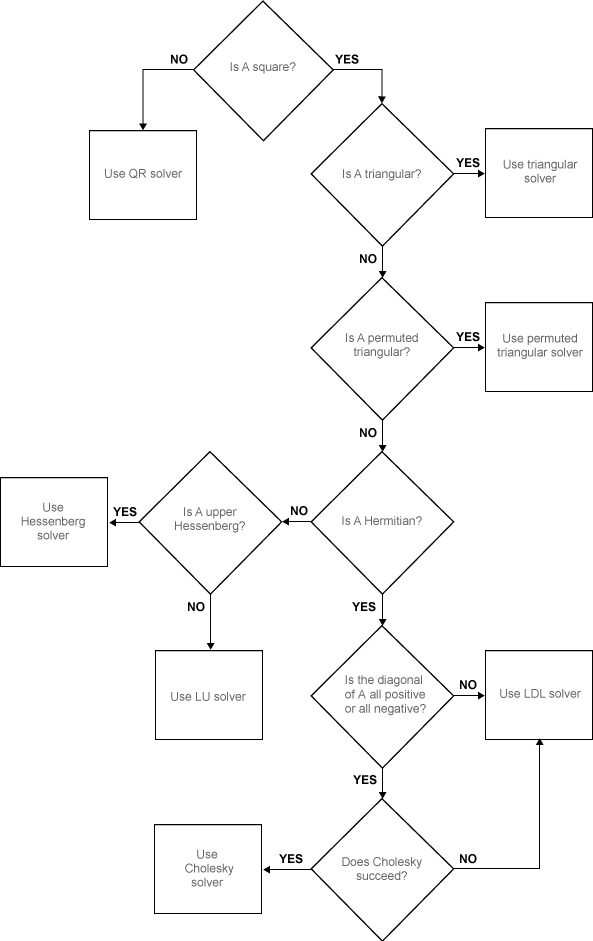
\includegraphics[scale = 0.4]{mldivide_full.png}
        \caption{MATLAB mldivide full matrix flowchart}
    \end{figure}
    
    \newpage
    If A or b are sparse, then this flowchart is used instead:\newline
    
    \begin{figure}[h]
        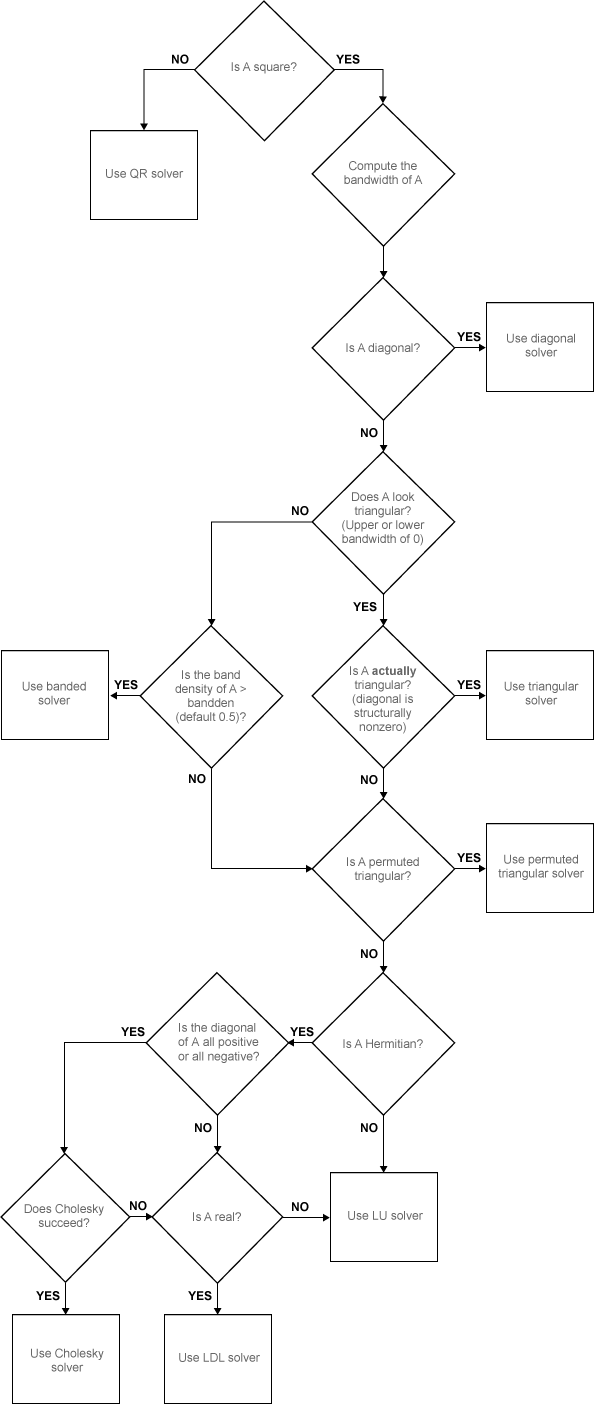
\includegraphics[scale = 0.4]{mldivide_sparse.png}
        \caption{MATLAB mldivide sparse flowchart}
    \end{figure}

    \end{flushleft}
    \newpage
    \item $b^\prime/A$
    \begin{flushleft}
   Accoriding to the official MATLAB R2018b documentation located at:
    https://www.mathworks.com/help/matlab/ref/mrdivide.html \newline
    "x = B/A solves the system of linear equations x*A = B for x." By transposing the vector b, the number of columns of the two matrices will be equal. Therefore, we are effectively allowing this operation to take place for any non-singular inputs.
    \newline
    \end{flushleft}
    \item $A/b$
    \begin{flushleft}
    Accoriding to the official MATLAB R2018b documentation located at:
    https://www.mathworks.com/help/matlab/ref/mrdivide.html \newline
    "x = B/A solves the system of linear equations x*A = B for x. The matrices A and B must contain the same number of columns." Since B has only 1 column and A is square, this operation only works if A is a 1x1 matrix.
    \newline
    \end{flushleft}
    \item $A\backslash b$ vs. inv$(A) *b$
    \begin{flushleft}
    $A\backslash b$ involves partial pivoting and specialized algorithms dependent upon the form of A. As was shown in a previous exercise, pivoting decreases the number of FLOPs needed and would be more efficient than simply solving using inv$(A) *b$.
    \end{flushleft}
\end{enumerate}
\end{flushleft}

\newpage
\item[3.] Consider Gaussian elimination with partial pivoting. Recall
the growth factor $g _ { P P } = \frac { \max _ { i , j } \left| u _ { i j } \right| } { \max _ { i , j } \left| a _ { i j } \right| }$ measures the degree of stability of the elimination process.\newline
Consider matrices of the form
$$A = \left[ \begin{array} { c c c c c } { 1 } & { } & { } & { } & { 1 } \\ { - 1 } & { 1 } & { } & { } & { 1 } \\ { - 1 } & { - 1 } & { 1 } & { } & { 1 } \\ { - 1 } & { - 1 } & { - 1 } & { 1 } & { 1 } \\ { - 1 } & { - 1 } & { - 1 } & { - 1 } & { 1 } \end{array} \right]$$

\begin{enumerate}
    \item Experiment with solving $n \times n$ systems of equations $Ax = b$ by GEPP. You should observe that the result of elimination are meaningless (slight perturbation might be necessary to observe the worst behavior).\newline
    \begin{flushleft}
    The code below is used to calculate the residuals of a random vector of a given dimension:
    \end{flushleft}
    \begin{lstlisting}[mathescape=true]
    function residual = GEPP_Experiment (n)
        a = eye(n,n) - tril(ones(n,n),-1);
        a(:,n) = 1;
        
        x = randn(n,1);
        b = a*x;
        
        [lpp,upp,ppp]=lu(a);
        xpp = upp\(lpp\(ppp*b));
        
        residual = b - a*xpp;
        return
    end
    \end{lstlisting}
    \vspace{.15in}
    \begin{flushleft}
    If $n$ is small enough, we notice that the residual will consistently be 0. We can run the program 100 times for each dimension of $A$ and calculate the average infinite norm of the residual.
    \newline
    \end{flushleft}
    \begin{lstlisting}[mathescape=true]
    function average = GEPP_average(n)
        sum_r = 0;
        for i = 1 : 10
            sum_r = sum_r + norm(GEPP_Experiment(6),inf)
        end
        average = sum_r/100;
        return
    end
    \end{lstlisting}
    \begin{center}
    \begin{tabular}{ |c|c|c|c| } 
    \hline
    size(A) & Avg($\|\|_\infty$) \\
    \hline
    1   &   0\\
    2   &   0\\
    3   &   1.5488e-16\\ 
    4   &   3.5583e-16\\
    5   &   6.3310e-16\\
    6   &   1.4118e-15\\
    7   &   4.5880e-15\\
    8   &   5.7337e-15\\
    9   &   1.0657e-14\\
    10  &   2.2321e-14\\
    25  &   6.8911e-10\\
    50  &   0.0278\\
    75  &   23.9770\\
    \hline
    \end{tabular}
    \end{center}
    \vspace{.15in}
    \begin{flushleft}
    As we can see, the residual starts out at zero for small matrices and becomes significant once A becomes closer to a $50 \times 50$ matrix. This shows that the result of elimination essentially become meaningless as the large error in the first variable become propagated to every other during back substitution.
    \newline
    \end{flushleft}
    \newpage
    \item Show that the growth factor is of the order of $2^{n-1}$\newline
    \begin{flushleft}
    Let A be of the form given above with size $n \times n$.
    $$A = \left[ \begin{array} { c c c c c } { 1 } & { } & { } & { } & { 1 } \\ { - 1 } & { 1 } & { } & { } & { 1 } \\ { - 1 } & { - 1 } & { 1 } & { } & { 1 } \\ { \vdots } & { \vdots } & { \vdots } & { \ddots } & { 1 } \\ { - 1 } & { - 1 } & { - 1 } & { \cdots } & { 1 } \end{array} \right]$$
    Gaussian elimination with partial pivoting involves no pivoting as $A$ is already in the desired form. To start the Gaussian elimination, we add the first row to the every other to produce zeroes in the first column and 2's in the last column as follows:
    $$A^\prime = \left[ \begin{array} { c c c c c } { 1 } & { } & { } & { } & { 1 } \\ { 0 } & { 1 } & { } & { } & { 2 } \\ { 0 } & { - 1 } & { 1 } & { } & { 2 } \\ { \vdots } & { \vdots } & { \vdots } & { \ddots } & { 2 } \\ { 0 } & { - 1 } & { - 1 } & { \cdots } & { 2 } \end{array} \right]$$
    This process is repeated by adding the second row to every row below it to create zeros in the second column and 4's in last column. Therefore after repeating the process for k rows, we get zeros below the diagonal in the first k columns and $2^{k-1}$ in the remaining row in the last column. Completing the process for all n rows gives us the final form:
    $$U = \left[ \begin{array} { c c c c c } { 1 } & { } & { } & { } & { 1 } \\ { 0 } & { 1 } & { } & { } & { 2 } \\ { 0 } & { 0 } & { 1 } & { } & { 4 } \\ { \vdots } & { \vdots } & { \vdots } & { \ddots } & { \vdots } \\ { 0 } & { 0 } & { 0 } & { \cdots } & { 2^{n-1} } \end{array} \right]$$
    We can then easily calculate the growth factor as follows: $g _ { P P } = \frac { \max _ { i , j } \left| u _ { i j } \right| } { \max _ { i , j } \left| a _ { i j } \right| }$ = $\frac{2^{n-1}}{1}$ = $2^{n-1}$
    \newline
    \end{flushleft}
    \newpage
    \item Modify the \texttt{pivot.m} to calculate three backward error estimates for this problem.
    \begin{flushleft}
    The code was modified to initialize the matrix $A$ with the same form used in this problem. The specific modification was to print out the backward error vectors and to include the following lines of code to hard-code the initial matrix:
    \begin{lstlisting}
        a = eye(n,n) - tril(ones(n,n),-1);
        a(:,n) = 1;
    \end{lstlisting}
    The program calculates various types of backward errors including the true backward error and the component-wise relative backward error for both GEPP and GECP algorithms. The relevant graphs generated are included at the end of this file. The various backwards errors calculated are vectors representing the true backward error (macheps*$\|A*x-b\| / (\|A\| \|x\|$ ) and the component-wise relative backward error for both GEPP and GECP, denoted in the code as bndpp3, bndpp5, bndcp3, and bndcp5, respectively.
    \newline
    \end{flushleft}
    \item Use Hager's algorithm to estimate condition number and compare with Matlab's \texttt{cond(A)} and \texttt{rcond(A)} functions.\newline
    
    \begin{flushleft}
    According to the official MATLAB R2018b documentation located at: https://www.mathworks.com/help/matlab/ref/cond.html \newline
    "cond(A) returns the 2-norm condition number for inversion, equal to the ratio of the largest singular value of A to the smallest."
    \newline
    
    According to the official MATLAB R2018b documentation located at: https://www.mathworks.com/help/matlab/ref/rcond.html \newline
    "rcond(A) returns an estimate for the reciprocal condition of A in 1-norm."
    \newline
    
    The following table was created for comparing the condition numbers for various dimensions of A.
    \newline
    
    \end{flushleft}
    \begin{center}
    \begin{tabular}{ |c|c|c|c| } 
    \hline
    size(A) & Hager & cond(A) & rcond(A) \\
    \hline
    1   &   1   &   1   &   1\\
    2   &   2   &   1   &   0.5\\
    3   &   3   &   1.414   &   0.333\\ 
    4   &   4   &   1.811   &   0.25\\
    5   &   5   &   2.224   &   0.2\\
    6   &   6   &   2.646   &   0.167\\
    7   &   7   &   3.075   &   0.143\\
    8   &   8   &   3.509   &   0.125\\ 
    \hline
    \end{tabular}
    \end{center}
    \vspace{.15in}
    \begin{flushleft}
    Based on this data, we can hypothesize that \texttt{Hager(A)} $\geq$ \texttt{cond(A)} $\geq$ \texttt{rcond(A)} for any size A of the given form. It appears that Hager's algorithm is extremely close to the 1-norm condition number and so \texttt{rcond(A)} is the reciprocal of that condition number. The code used to calculate the condition number using Hager's algorithm is included here:\newline
    \end{flushleft}
    \begin{lstlisting}
function cond = condition_hager (n)
  i1 = -1;
  c1 = 0.0;
  a = eye(n,n) - tril(ones(n,n),-1);
  a(:,n) = 1;
  b(1:n,1) = 1.0 / n;

  while ( 1 )
    b = a \ b;
%   c2 is the norm of the inverse
    c2 = sum ( abs ( b(1:n,1) ) );
    b = sign ( b );
    i = find ( b == 0.0 );
    b(i) = 1.0;
    b = a' \ b;
    
    max_index = 1;
    for i = 2 : n
      if ( abs ( b(max_index) ) < abs ( b(i) ) )
        max_index = i;
      end
    end
    i2 = max_index;

    if ( 1 <= i1 )
      if ( i1 == i2 || c2 <= c1 )
        break
      end
    end

    i1 = i2;
    c1 = c2;
    b(1:n,1) = 0.0;
    b(i1,1) = 1.0;
  end
  cond = c2 * norm ( a, 1 );
  return
end
\end{lstlisting}

\end{enumerate}
\end{enumerate}

\newpage
\begin{landscape}
\begin{figure}[h]
        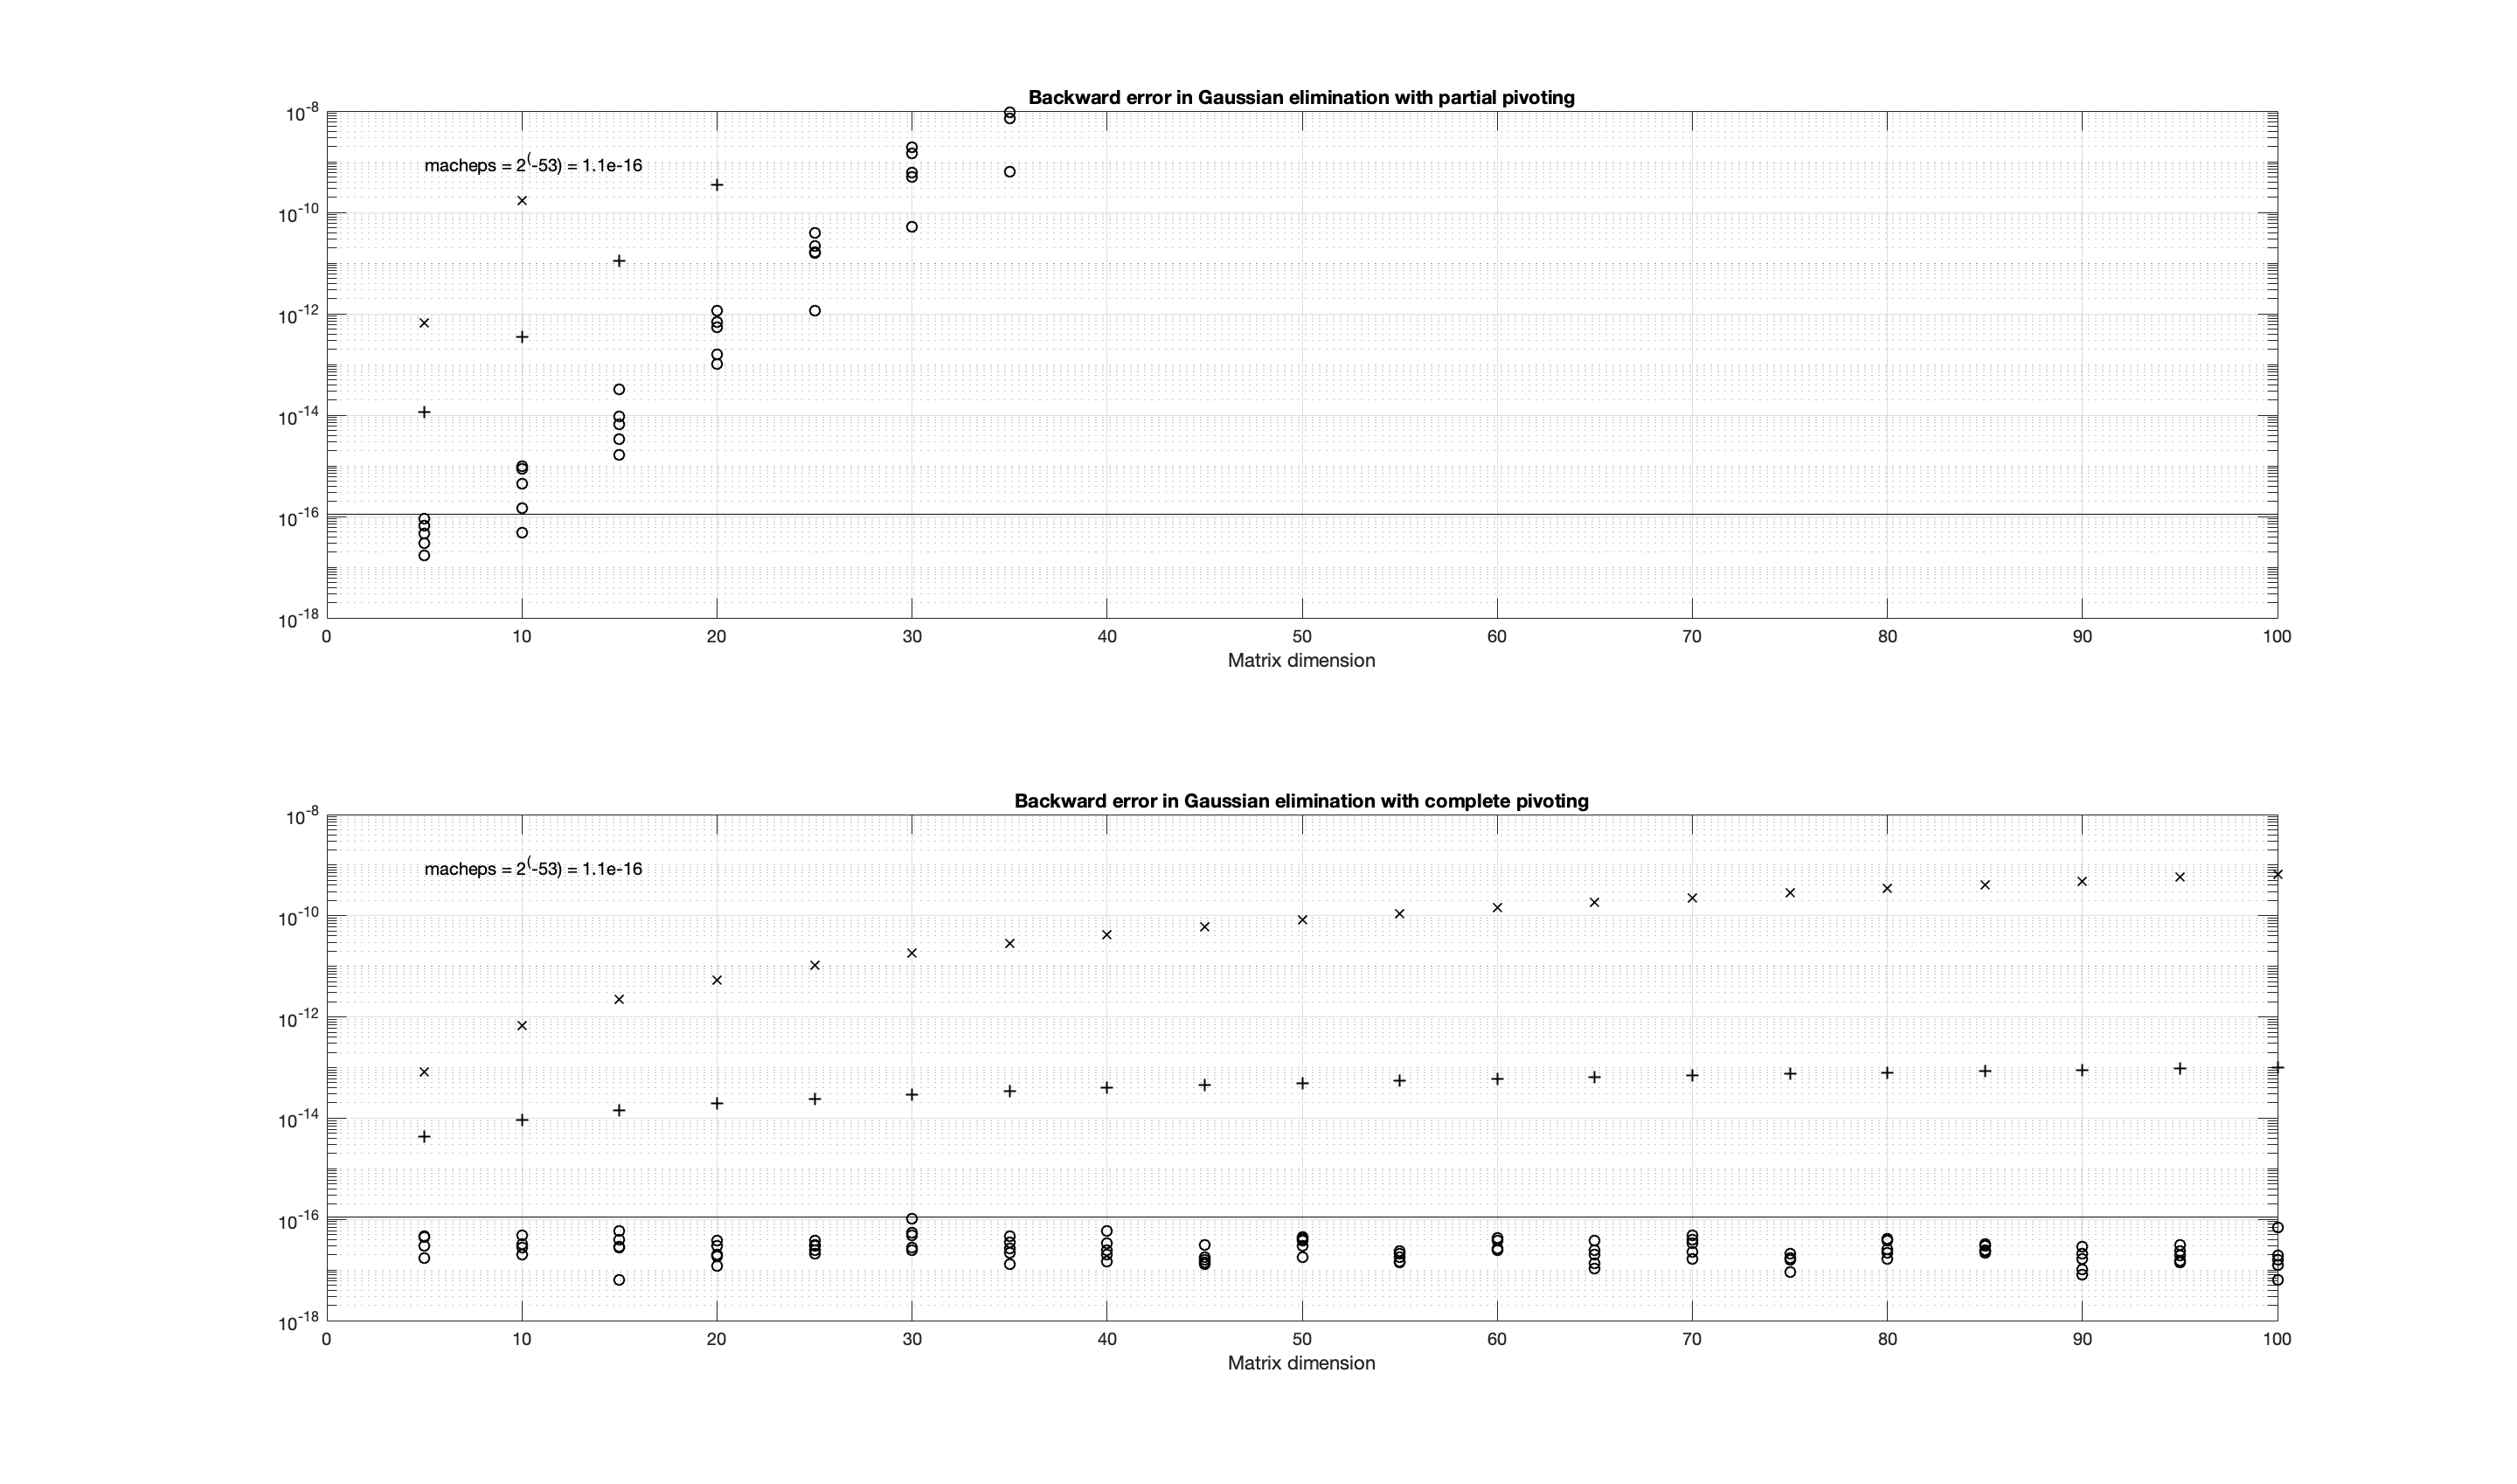
\includegraphics[scale = 0.25]{BE_GEPP_GECP.png}
        \caption{Backward Errors in GEPP \& GECP}
\end{figure}
\end{landscape}

\newpage
\begin{landscape}
\begin{figure}[h]
        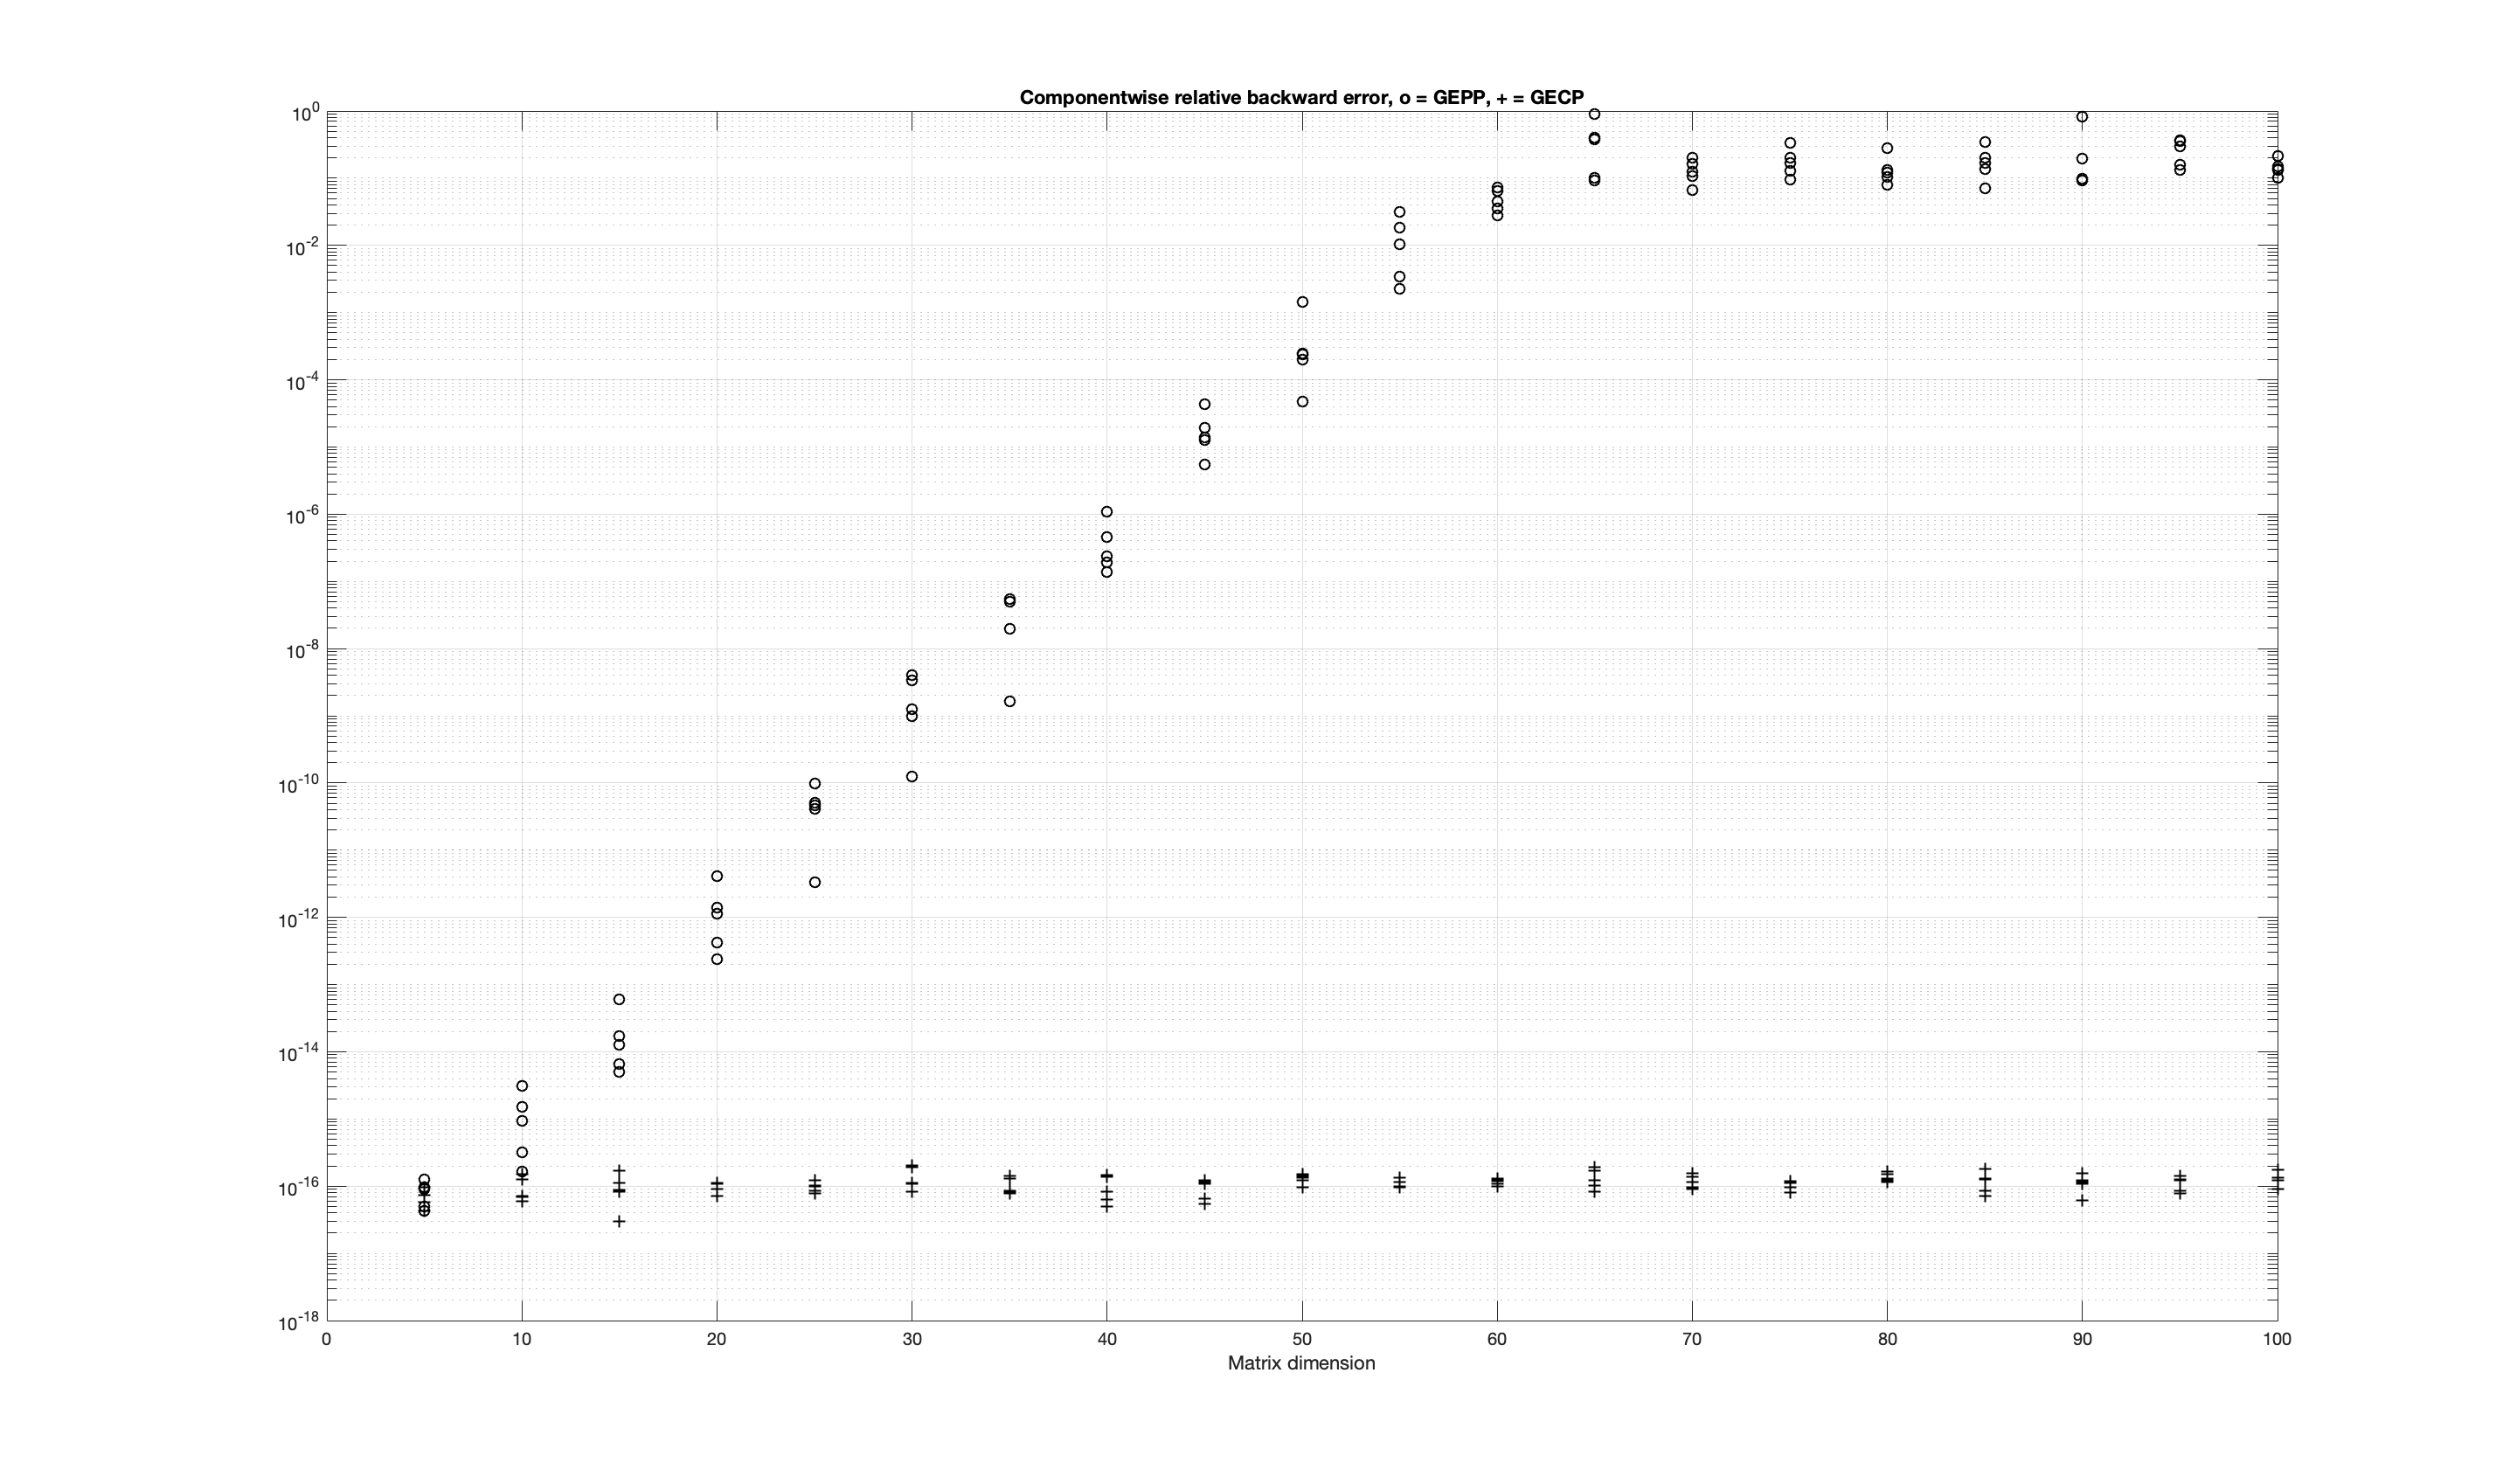
\includegraphics[scale = 0.25]{CWRBE.png}
        \caption{Component-wise Relative Backward Error}
\end{figure}
\end{landscape}

\newpage
\begin{landscape}
\begin{figure}[h]
        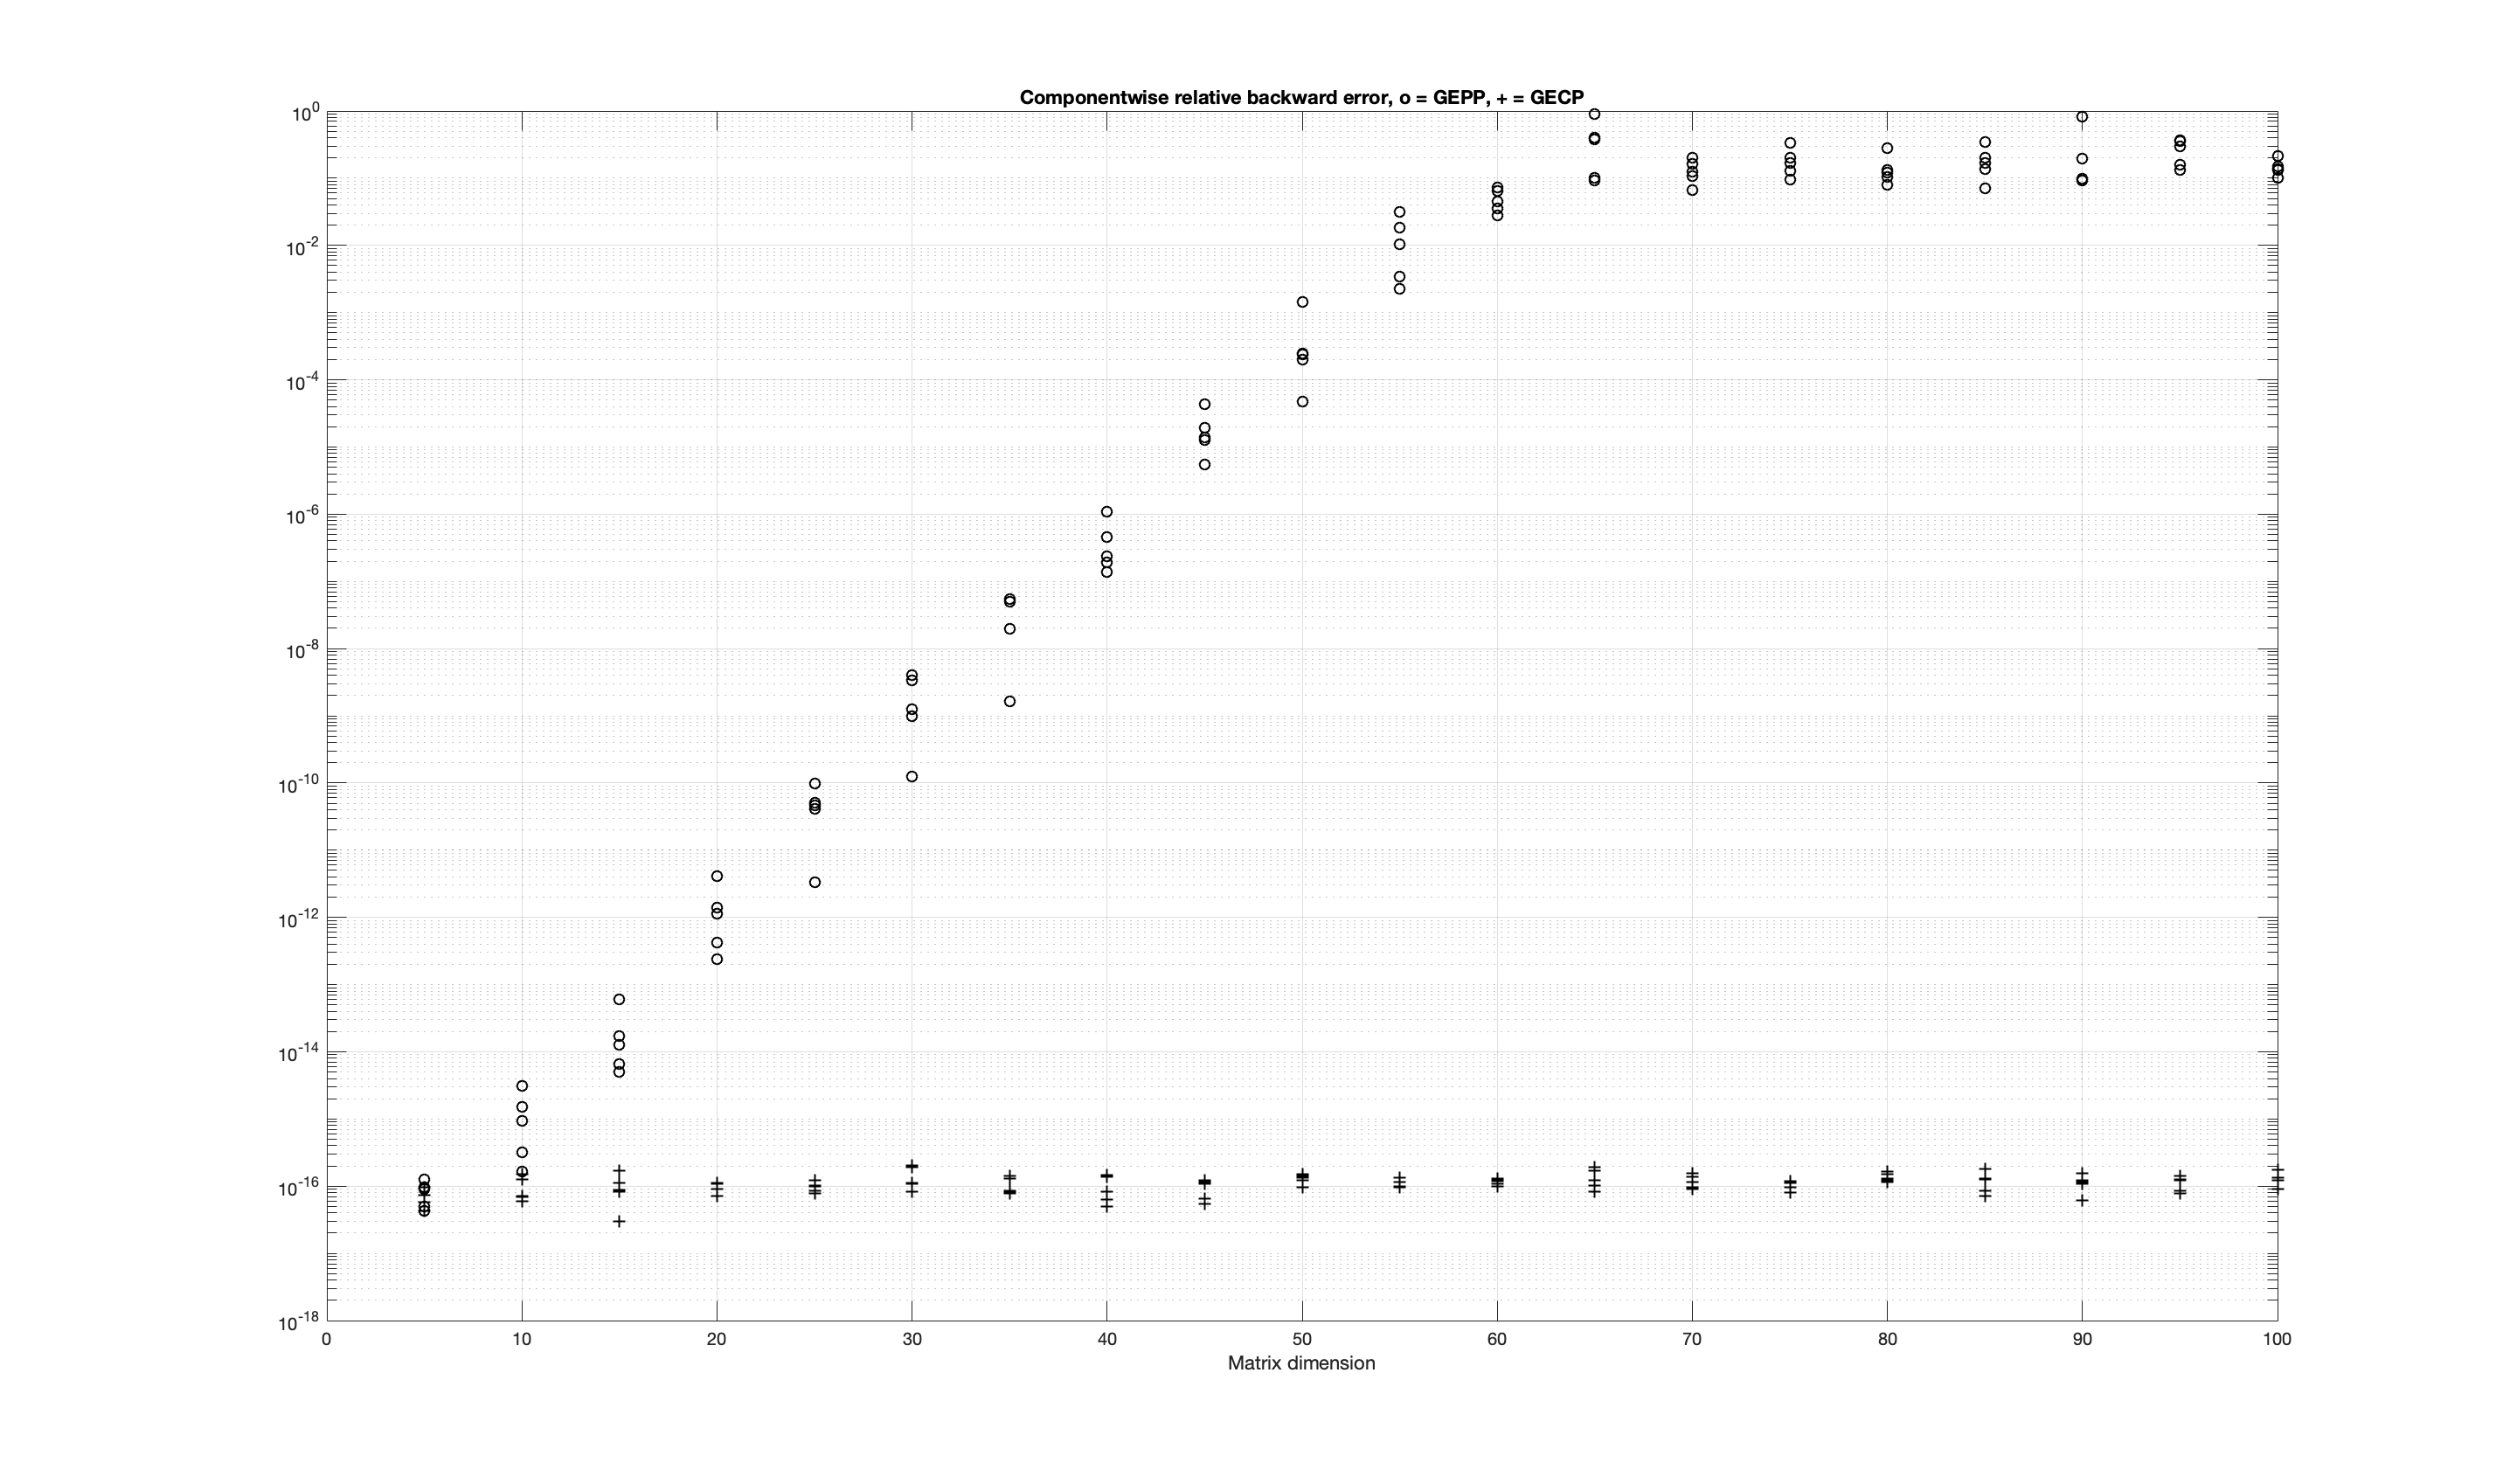
\includegraphics[scale = 0.25]{CWRBE.png}
        \caption{Component-wise Relative Backward Error after Iter Ref}
\end{figure}
\end{landscape}

\end{document}